\documentclass[11pt]{article}
\usepackage{geometry}                % See geometry.pdf to learn the layout options. There are lots.
\geometry{letterpaper}                   % ... or a4paper or a5paper or ... 
%\geometry{landscape}                % Activate for for rotated page geometry
%\usepackage[parfill]{parskip}    % Activate to begin paragraphs with an empty line rather than an indent
\usepackage[pdftex]{graphicx}
\usepackage{amssymb}
\usepackage{epstopdf}

\usepackage[T1]{fontenc}
\usepackage[scaled=0.8]{beramono}

%\DeclareGraphicsRule{.tif}{png}{.png}{`convert #1 `dirname #1`/`basename #1 .tif`.png}
\usepackage{listings} 

\lstset{%
  frame=none,
  xleftmargin=5pt,
  stepnumber=1,
  numbers=left,
  numbersep=5pt,
  numberstyle=\ttfamily\tiny,
  belowcaptionskip=\bigskipamount,
  captionpos=b,
  escapeinside={<|}{|>},
  tabsize=2,
  emphstyle={\bf},
  commentstyle=\it,
  stringstyle=\mdseries\ttfamily,
  showspaces=false,
  keywordstyle=\bfseries,
  morekeywords={in,do,print},
  columns=flexible,
  basicstyle=\sffamily,
  showstringspaces=false,
  morecomment=[l]\%,
}

\lstdefinelanguage{Enso}{%
  numbers=none,
  sensitive=true,
  morecomment=[l]{//},
  morecomment=[s]{/*}{*/},
  morestring=[b]",
  emphstyle={\bf},
  commentstyle=\it,
  stringstyle=\mdseries\ttfamily,
  showspaces=false,
  basicstyle=\ttfamily,
  morekeywords={schema,type},
  keywordstyle=\bfseries,
  columns=flexible,
  showstringspaces=false,
  morecomment=[l]\%,
}

\newcommand{\C}{\lstinline}

\lstset{language=Enso}

\newcommand{\Enso}{Ens\={o}}

\title{
\includegraphics[scale=0.25]{enso.jpg}\\\Enso}
\author{William R. Cook and Tijs van der Storm}
%\date{}                                           % Activate to display a given date or no date

\begin{document}
\maketitle

\begin{abstract}
\Enso\ is a new approach to software development
based on integrated executable specification languages.
An executable specification language (ESL) allows programmers
to specify \textit{what} should be computed while
relying on the language implementation to determine
exactly \textit{how} the computation should be performed.
Examples of ESLs include grammars, spreadsheets, 
attribute grammars, database queries, 
access control policies, and makefiles.
In its goals, \Enso\ is closely related to 
domain-specific language (DSL) workbenches and 
model-driven development (MDD) systems. \Enso\ differs
from existing systems in several ways.
\Enso\ focuses on language \textit{interpreters}
rather than language embedding or transformation/compilation. 
These interpreters are examples of \textit{generic operations},
which are operations that are guided by an ESL. 
To integrate multiple ESLs and implement cross-cutting aspects,
\Enso\ uses interpreter wrapping and composition.
\Enso\ supports both textual and graphical presentations.
\Enso\ is implemented using itself with a tight bootstrap process
and dynamic typing. 
\Enso\ will ship with a collection of
extensible languages for data modeling,
web programming, GUI development, access control, database access,
software evolution, among others. 
\end{abstract}

The concept of an \textit{executable specification language} (ESL) is
to many computer scientists an oxymoron. The key characteristic
of a specification language is that it specifies \textit{what} should
be computed without saying \textit{how} to compute it.
General-purpose specification languages, including Z and B,
are far too expressive to admit any direct execution of specifications.
However, by restricting the specification language to
describe what should be computed within a limited scope of
problems, it is possible to create useful languages that specify
what should be computed, while still supporting efficient
and fully-automatic execution.

Well-known examples of ESLs include grammars, spreadsheets,
attribute grammars, database queries,
access control policies, and makefiles. These are not normally
considered to be specification languages, but we believe the term
applies because they describe what should be computed rather
than how to compute the results.
A grammar specifies
what language should be recognized, but not how to recognize it.
Spreadsheets and attribute grammars give
equations that must be satisfied, but do not specify order of execution.
Access control policies specify the conditions under which
a user is allowed to perform an operation on an object, but
does not specify how to efficiently enforce the policy everywhere
in the program that the rule might apply. Different languages
provide different degrees of abstraction away from the raw ``how''
of computation, and there is no absolute objective measure
of this quality. 

In its goals, \Enso\ is closely related to
domain-specific language (DSL) workbenches and
model-driven development (MDD) systems. [describe them?]

We avoid the phrase ``domain specific'' because the word
``domain'' is ambiguous and potentially misleading. We believe that
executability is the essential requirement.
Restricting a language to a special purpose, or domain of
application, is the means to achieve this goal
but is not the goal itself. Some languages, like datalog
and attribute grammars, are executable but they are
sufficiently general-purpose that it seems an abuse of terminology
to call them domain specific. As another example, consider
that the relational calculus and the relational algebra are
both domain-specific, but the relational algebraic is more specific
about how a query will be computed. Given the right context,
we do believe that ``domain-specific'' is a reasonable
description for most ESLs.

Similarly, we also avoid the word ``declarative''.
Although it is often used to mean
``specifying what to compute, not how to compute it'',
it also means the absence of imperative
effects, especially mutable state and assignment.
This brings up the question of whether statecharts
can be considered a declarative language, because they
have an inherent notion of mutable state.
On the other hand functional languages, including
Haskell, are always described as declarative, but we do not
consider them specification languages because
they specify how to compute
a result rather than describing what result is desired.
Thus we prefer ``specification language'' over
``declarative language''.

The word ``model'' is a natural name for specification
written in an executable specification language. This usage
ties nicely with the idea that a model is a schematic description
of some phenomenon of interest. This usage
should not be confused with the usage of ``model'' in logic,
where it describes a structure that satisfies a set of formula.
In the software world, ``model'' has come to mean a graphical
description, or picture, as in the Unified Modeling Language (UML).
However, we use the term ``model'' to refer to either textual
or graphical presentations of a specification.

\Enso\ differs from existing systems in several ways.

\Enso\ is based on interpretation rather than code generation. 
While it is possible to define transformations that generate code
in conventional languages, this is rarely (if ever) done in \Enso.
Instead all structural descriptions and transformations are 
interpreted dynamically. Although the current incarnation of \Enso\
does not include it, we have previously demonstrated that partial
evaluation can be applied to \Enso-style interpreters to automatically
generate efficient code.

To integrate multiple ESLs and implement cross-cutting aspects,
\Enso\ uses interpreter wrapping and composition.

\Enso\ supports both textual and graphical presentations.

\Enso\ is implemented using itself with a tight bootstrap process
and dynamic typing. 

\Enso\ will ship with a collection of
extensible languages for data modeling,
web programming, GUI development, access control, database access,
software evolution, among others. 

What follows is a rapid introduction to the concepts and use of
\Enso. To avoid too many digressions, 
the many connections between \Enso\ and existing approaches,
including programming models
(model-driven, object-oriented, polytypic, functional, constraint-based), theory (dependent types, coalgebra, category theory),
and related ideas (relational databases, domain-specific languages)
are discussed in Section~\ref{relatedwork}.

\section{Data Description}

One of the most important kinds of ESL is the 
\textit{data description language}. The intent of a data
description language is to specify the structure and
behavior of data. The history of the development of data
description covers much of the history of programming languages themselves.

Type systems in programming languages are
well-known examples of data description languages, including
records/arrays/unions in Pascal or C, or sums of products
data types in Haskell and ML. These systems are very useful
for describing the structure of data. Such structures are 
important because they can be checked automatically via a
static type system. Data types are specifications because they
define what data is needed, not how to implement it.

The problem is that the actual data in a system 
almost always obeys additional invariants and behaviors that
are not expressible in a structural data description. 
Dynamic languages also have this problem, because they 
provide only a single universal type that is flexible 
enough to express any desired data. 

\textit{Abstract data types} (ADTs) and \textit{objects} 
wrap raw structures with a 
set of procedures that enforce invariants and supply 
higher-level operations or behaviors. The difference is
that ADTs manage a set of values with hidden representation,
while objects bundle the procedures into the actual values
themselves. Despite the differences, ADTs and objects are
similar in their level of description.

One problem with both ADTs and objects is that they are
both fundamentally \textit{operational}. That is, they define \textit{how}
to implement the desired properties of data, rather than
specifying \textit{what} properties are needed. If an invariant
can be affected by multiple operations in an ADT, then code
must be written to check or enforce the invariant in multiple places.
In many cases the invariants span multiple individual data
items, so code must be coordinated between data abstractions. 
One common example is the owner/items pointers that must
be coordinated to ensure consistency of a hierarchical structure.

A second problem with implementation-oriented descriptions of
data types is that they do not scale well when an application has 
dozens or hundreds of different data types,
each with specific behavior and named properties but also many common properties and
behaviors. Global behaviors like caching, persistence, security,
and common repeated patterns like cached computed attributes and
bidirectional relationships cannot be expressed as libraries or
reusable class definitions. These concepts can easily be described
as \textit{design patterns}, but the programmer must still implement
them in each specific instance, in some cases hundreds or 
thousands of times! It becomes impossible to change such
pervasive design decisions after the code is written.

One reason for this is that these 
features require quantification over \textit{names} and/or \textit{types}
rather than values. [Example is bidirectional relationships]. 
In sophisticated object-oriented frameworks,
reflection is often used to implement these general features. However,
reflection is quite complex to use. It is a very powerful tool to
solve what might otherwise be relatively simple problems.

If ADTs and objects are not sufficient, what about about existing
specification languages?
Maude and Alloy are examples of the alternative: they define 
properties of data. [more on these? basically they are good, but they
aren't as ``executable'' as we would like].

The question, then, is whether it is possible to express useful global
and local properties of data, while still allowing pervasive strategies
for implementing the data and its properties. We believe that there
are several approaches that make sense, including entity-relationship
modeling, attribute grammars, and excel-style spreadsheets. 

\Enso\ does \textit{not} mandate
an particular data structuring mechanism. 
\Enso\ includes predefined data structuring techniques based on these 
models, but also mixes them together to make useful hybrids.
These were designed 
with specific purposes in mind: one is used in the implementation of
\Enso\ itself, and a variant is useful for access to relational databases.
But \Enso\ encourages users to define their own data description
strategy, or modify one of the basic ones to suit their needs. In
what follows we describe several of the data structuring techniques
that we have found useful in \Enso\ so far.

\subsection{Structures}

Structures in \Enso\ are a specialized kind of graph,
whose nodes are either primitive data or collections of observable
properties, whose values are either nodes or collections of nodes.
From a programming language viewpoint this may seem an odd 
choice for data representation. However, it is essentially the
Entity-Relationship (ER) model \cite{FOO}, also known as Information
Models \cite{FOO}, which is widely used in the design of relational databases
and is also the basis for Class Diagrams in 
the Unified Modeling Language (UML) \cite{FOO}, which 
describe the structure of networks of objects.
The key point is that structures in \Enso\ are 
viewed holistically as \textit{graphs}, not as individual values
or traditional sums-and-products data structures.

A structural description, or \textit{schema}, specifies some 
of the observable properties of structures. Schemas are used to
check the consistency structures. Some properties can be checked
while the structure is being created, but other can only be checked
once the structure is complete. \Enso\ allows modification of structures,
which is necessary to create cyclic graphs, but also allows 
valid structures to be sealed to prevent further changes.

\subsection{Schemas}

The following schema describes a collection of genealogy information:

\begin{verbatim}
schema GenealogySchema

  class Genealogy
    name: str
    members: Person*

  class Person
    name: str (key)
    birth: date
    female: bool
    father: Person?
    mother: Person?
\end{verbatim}

In a schema, a \textit{class} defines a kind of value, which is
followed by its properties or \textit{fields}. Each field has a name
and a type, where the type may be followed by \C|*| to indicate a 
many-valued field, or by \C|?| to indicate an optional value.
In this case, \C|Genealogy| has \C|members| which is a set of \C|Person|.
A \C|Person| has a \C|name| string, a \C|birth| date, and a \C|father| and \C|mother|,
which are optional \C|Person|s. The \C|father| and \C|mother| are optional
because every geneology is partial, so that not all fathers and mothers
can be included.

\subsection{Instances}

A particular collection of genealogy information, which conforms to the
above schema, might be written as follows:

\begin{verbatim}
Genealogy "Sam's Ancestors"
Person "Albert Snook"  11/1/89 male  +"Jane Snook" ^"Thomas Snook"
Person "Jane Snook"    3/17/48 female 
Person "Thomas Snook" 12/30/43 male 
\end{verbatim}

\subsection{Inverses}



\section{Interpretation}

Model -> Behavior

\subsection{Factories}

Structure are created by \textit{factories}, which create
and manage the nodes in the structure. The factory also
ensures that structures are distinct: a factory identifies the 
collection of nodes that belong to a graph, and any given node 
can only be connected to other nodes in the same graph, which were
created by the same factory.

In \Enso\ most properties of a structure are
checked when the structure is being created. In other words, 
the \textit{factory} that creates the structure is parameterized by a
schema, which the factory uses to check the legality of operations
on the objects it creates.

\section{Transformations}

TransformationModel -> (InstA -> InstB) \\
TransformationModel -> (InstB -> InstA)

Invertible transformations are used to map one structure into
another kind of structure, such that mapping can be inverted to 
(partially) recover the original structure from the result.
One common kind of transformation is called a \textit{grammar},
which is an invertible transformation between structures and text.
Text grammars are invertable because they can be used for parsing
and also rendering. Other transformations include Diagram grammars,
which map structures into diagrams, were edits on the diagram are
reflected in the original structure. Grammars that describe
the structure and behavior of user interfaces are used to generate
very natural applications.
Transformations are also used for querying, template processing, 
and serialization.

\subsection{Textual Grammars}


\subsection{Instantiation}


\section{QuadModel}


\begin{figure}[htbp]
\begin{center}
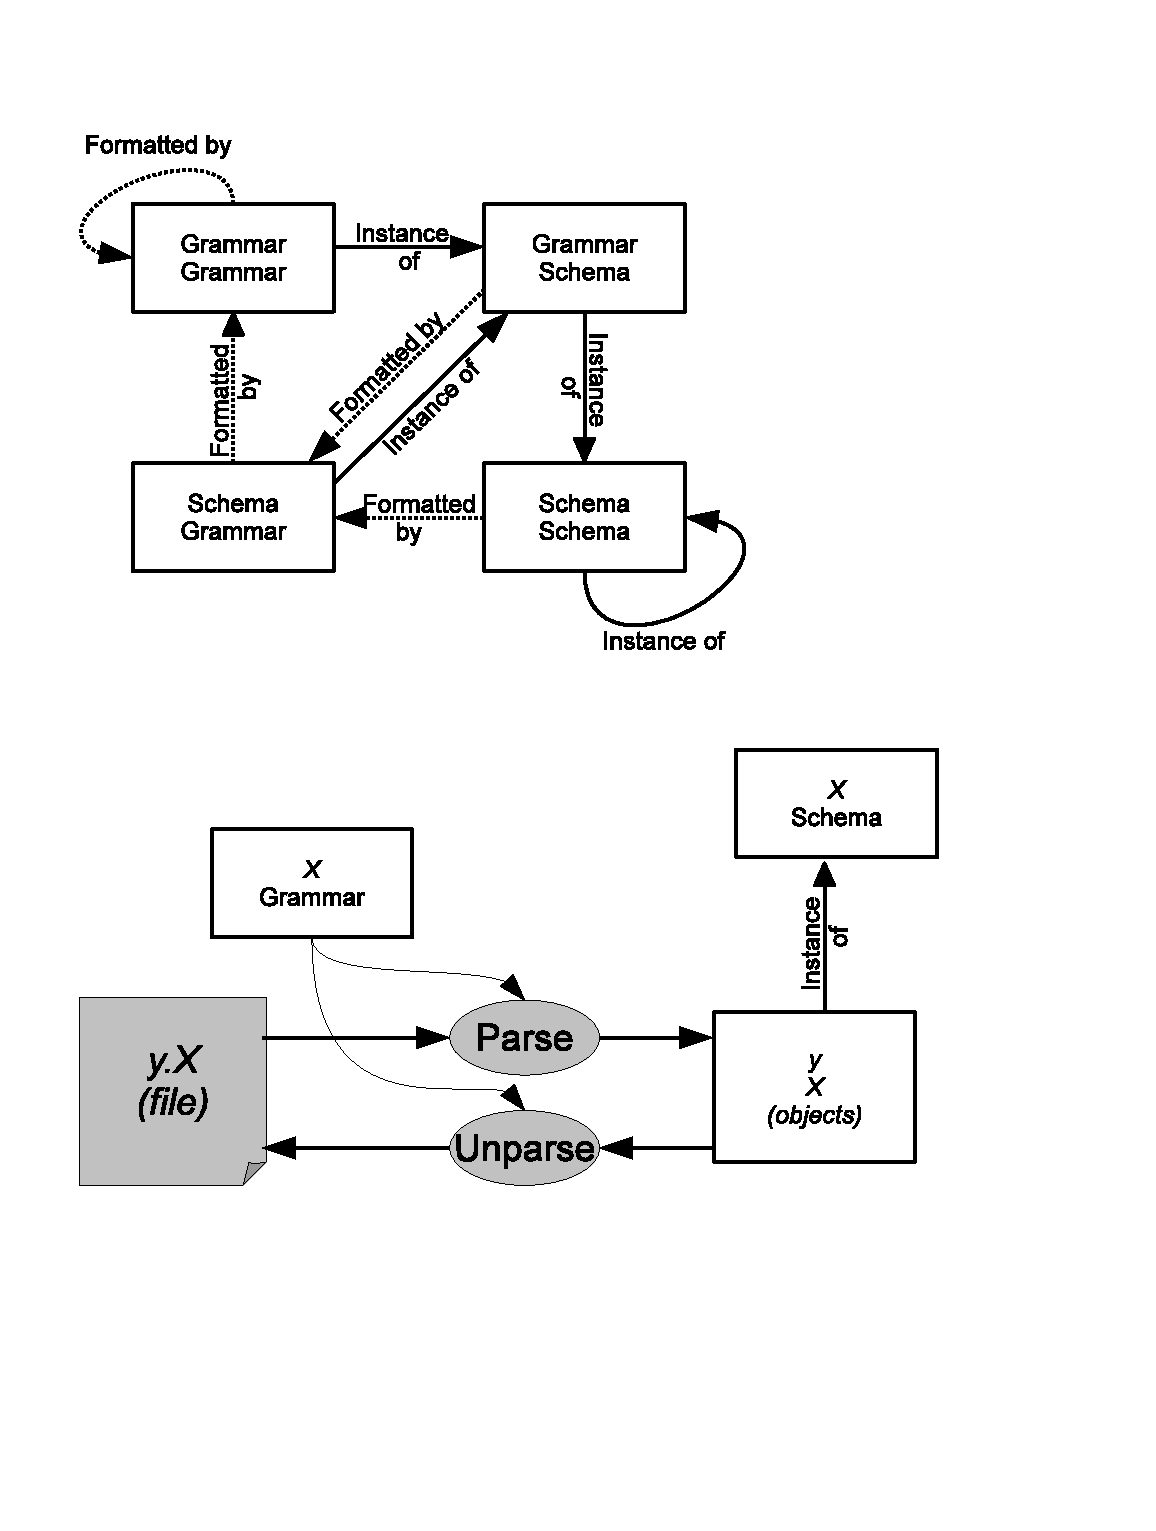
\includegraphics[scale=0.7]{QuadModel.pdf}
\caption{The four core schema and grammar models}
\label{default}
\end{center}
\end{figure}

\begin{figure}[htbp]
\begin{center}
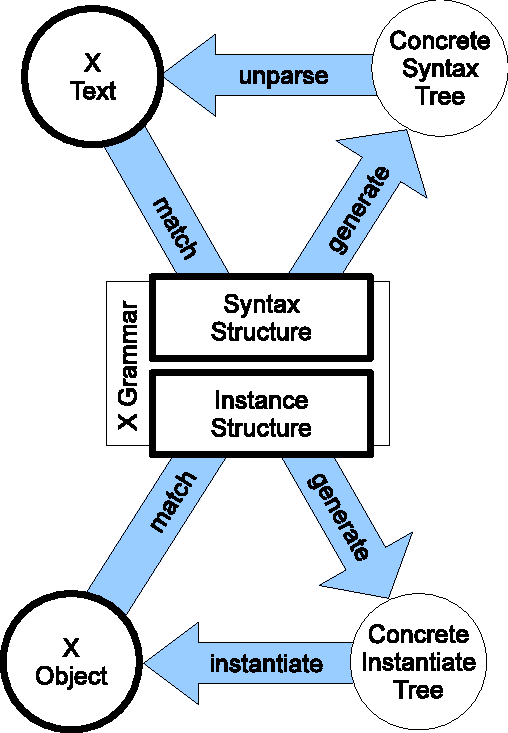
\includegraphics[scale=0.7]{ParseRender1.pdf}
\caption{Invertable grammar transformations}
\label{default}
\end{center}
\end{figure}
\begin{figure}[htbp]
\begin{center}
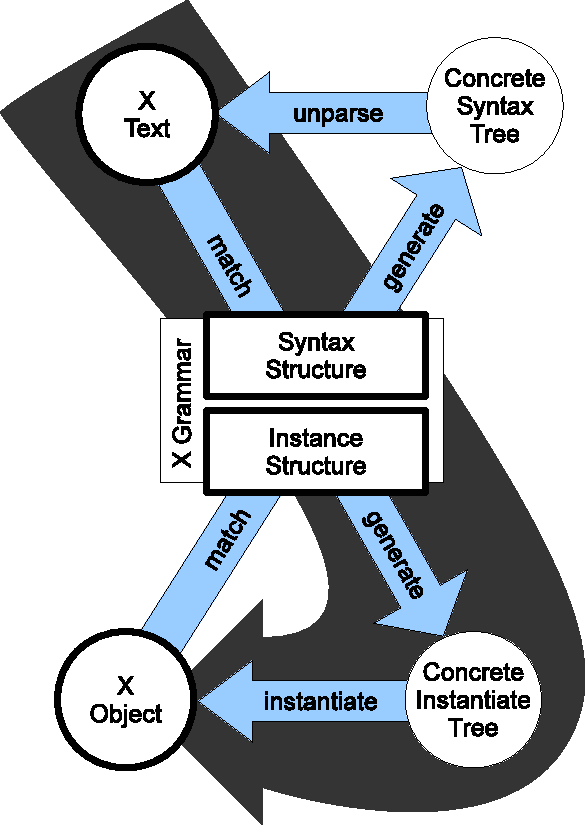
\includegraphics[scale=0.7]{ParseRender2.pdf}
\caption{Parsing matches \textit{syntactic structure} and generates \textit{instance structure}}
\label{default}
\end{center}
\end{figure}
\begin{figure}[htbp]
\begin{center}
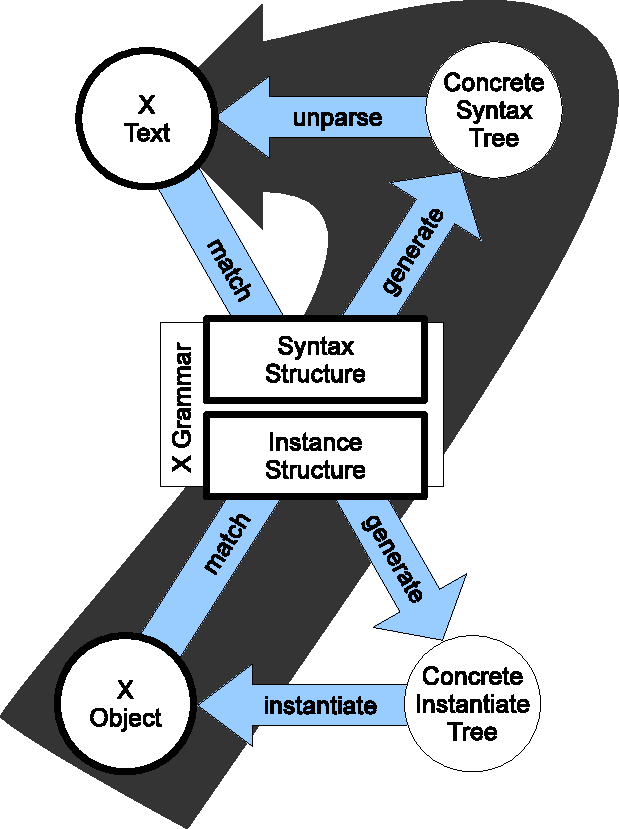
\includegraphics[scale=0.7]{ParseRender3.pdf}
\caption{Rendering matches \textit{instance structure} and generates \textit{syntactic structure}}
\label{default}
\end{center}
\end{figure}
\begin{figure}[htbp]
\begin{center}
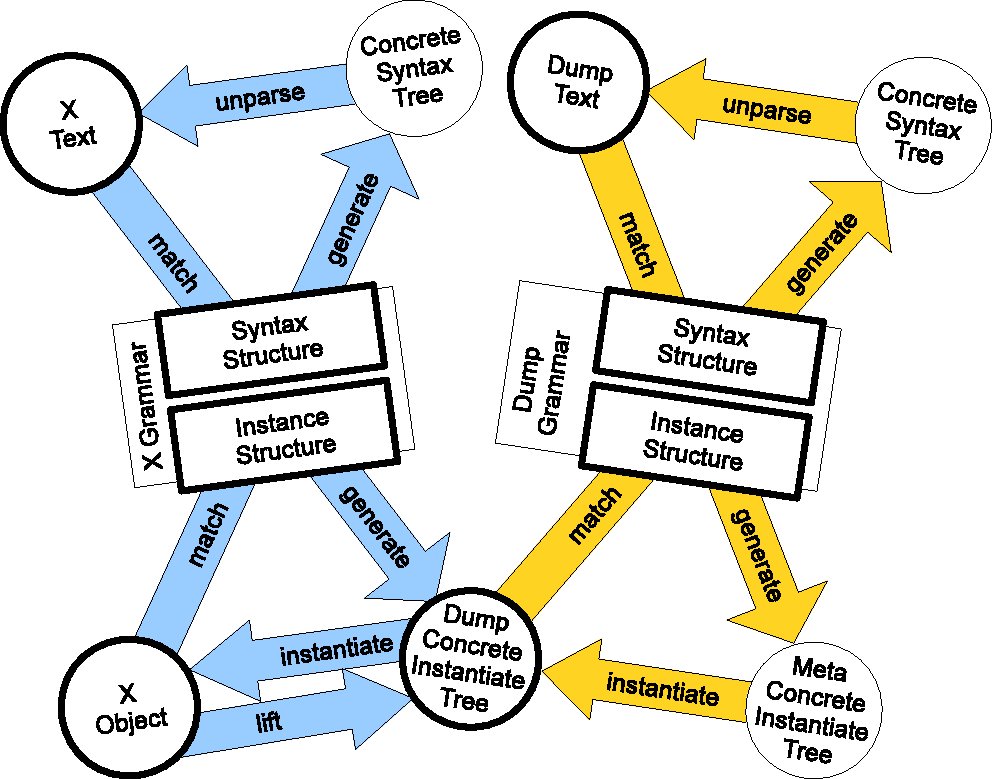
\includegraphics[scale=0.7]{ParseRender4.pdf}
\caption{Relationship between parsing and dumping}
\label{default}
\end{center}
\end{figure}
\begin{figure}[htbp]
\begin{center}
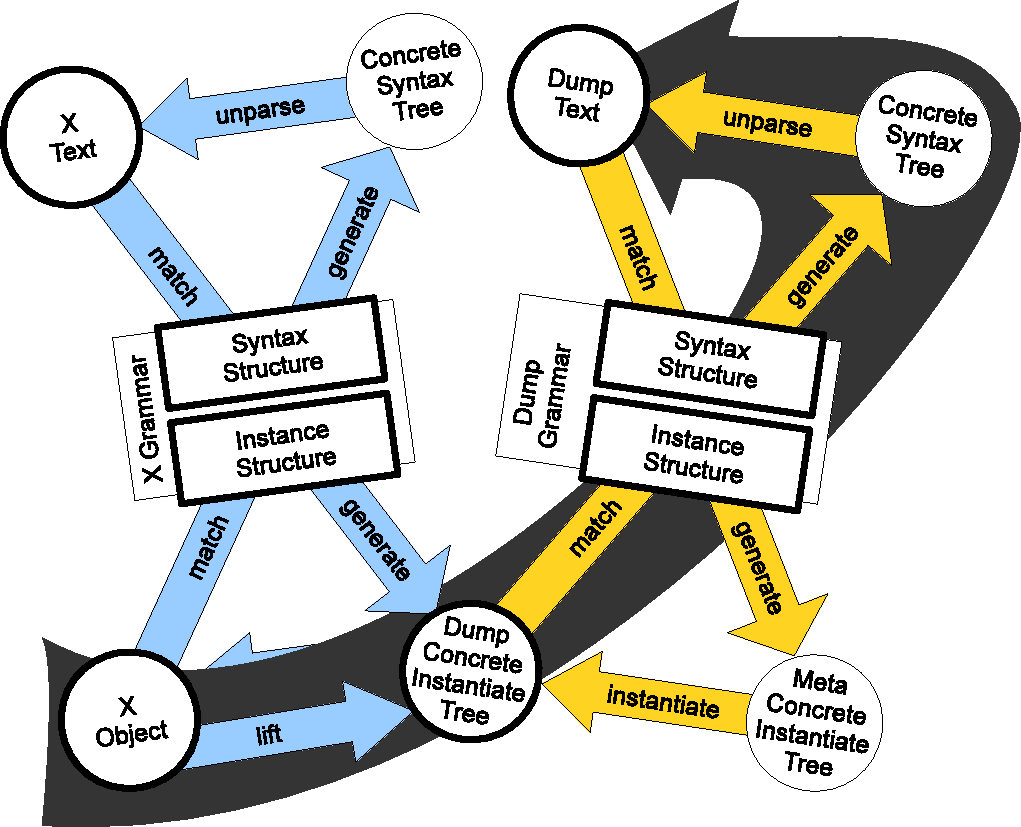
\includegraphics[scale=0.7]{ParseRender5.pdf}
\caption{Rendering to dump format}
\label{default}
\end{center}
\end{figure}

\begin{figure}[htbp]
\begin{center}
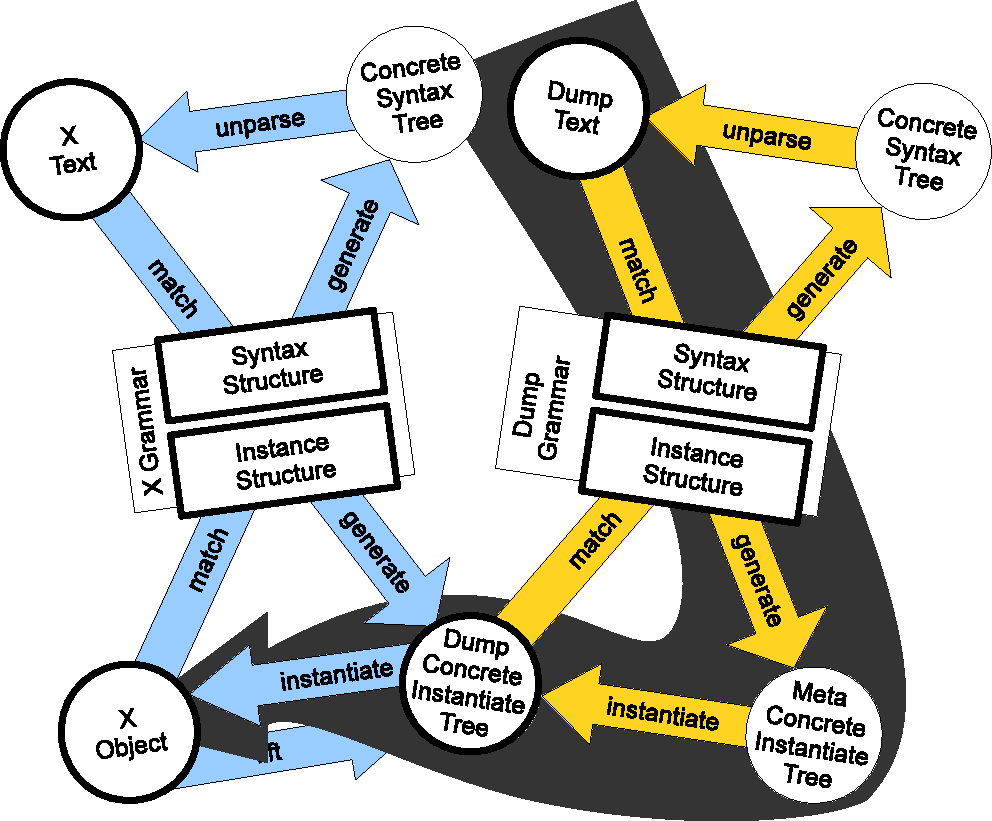
\includegraphics[scale=0.7]{ParseRender6.pdf}
\caption{Reading dump format to create objects}
\label{default}
\end{center}
\end{figure}


\section{Generic Operations}

Model -> Function

Operations can be guided by schemas or grammars, allowing highly
generic operations to be defined for comparison, differencing, 
merging, projecting and otherwise manipulating cyclic structures.
These operations are cyclic maps, which correspond to coinductive 
transformations.
Since schemas and transformations are also structures, they can
be merged and transformed using these same generic operations.
Transformations on schemas can be applied to instances, to support
upgrade and change management of data.
The resulting system supports powerful modularity constructs,
including feature modules, inheritance, and mixins.


\section{Implementation} 

\subsection{Requirements for a programming language}

The programming model is based on cyclic graphs.
Graphs are kept distinct from each other. That is,
each graph is considered a self-contained
artifact, without links or pointers to other graphs.

A natural way to create such graphs is with 
imperative effects.

This potentially requires more copying of data
than would be the case in tree-based representations.

To modify graphs, place-holder objects are useful,
as is the ability to ``become'' another object.

\subsubsection{Simple reflection}

Fields can be created dynamically and accessed with
``.'' notation or reflective access.

\begin{verbatim}
o.foo   == o.get("foo")
\end{verbatim}

Assignment to fields can be overriden
\begin{verbatim}
   o.bar = 3   ==> o.set("bar", 3)
\end{verbatim}

\subsection{Bootstrapping}


\section{Relationship to Other Approaches}
\label{relatedwork}

\Enso\ data is based on traditional 
entity-relationship (ER) models \cite{FOO},
which are also known as information models. 
ER models were the basis for class diagrams in UML.

In contrast to
object-oriented programming, \Enso\ is focused on holistic
object graphs, rather than individual objects. \Enso\ 
does allow data to include some behavior, for example constraints
and computed fields, but \Enso\ does not associated methods
with data objects.

In contrast to
most theories of functional programming, \Enso\ is based on
coalgebraic signatures rather than algebraic ones. In practice
this means that \Enso\ structures are cyclic graphs rather than
trees. Lazy functional languages can also represent cyclic 
structures, but the cycles are not observable.

\Enso\ supports controlled imperative effects. Objects are
mutable during construction or modification, while the data may be in an
inconstent state, but before it can be used it must be validated
and locked from further changes. This is similar to a transaction.


The rendering transformation is similar to Smaragdakis's notion of
Morphing \cite{Morphing} (or is it SafeGen?). 
However, \Enso\ generalizes the transformation
so that any kind of structure can be morphed into any other
kind of structure. On the other hand, \Enso\ is not statically
typed.

\Enso's generic operations are a form of polytypic programming, 
like Generic Haskell \cite{TH}. \Enso's operations can use
arbitrary meta-data, not just sum/product type structure.
On the other hand, \Enso's operations are not statically typed.
\Enso\ certainly shares the same goal to ``Write everything once''.

\subsection{Other Related Work}

Look up work on "instant-generics"


Eelco Lempsink, Sean Leather, and Andres L\&\#246;h. 2009. Type-safe diff for families of datatypes. In Proceedings of the 2009 ACM SIGPLAN workshop on Generic programming (WGP '09). ACM, New York, NY, USA, 61-72. DOI=10.1145/1596614.1596624 http://doi.acm.org/10.1145/1596614.1596624 

Dave Clarke, Michiel Helvensteijn, and Ina Schaefer. 2010. Abstract delta modeling. In Proceedings of the ninth international conference on Generative programming and component engineering (GPCE '10). ACM, New York, NY, USA, 13-22. DOI=10.1145/1868294.1868298 http://doi.acm.org/10.1145/1868294.1868298 

Data Representation Synthesis
Peter Hawkins, Alex Aiken, Kathleen Fisher, Martin Rinard, Mooly Sagiv. In Programming Language Design and Implementation (PLDI), ACM, 2011


[From CSSE 490 Model-Based Software Engineering: Transformational Programming
Shawn Bohner]
  Program Transformation Paradigms
  Interactive Program Transformation 
  Syntactic Abstractions in Intentional Programming 
  Simple Tree Parsing 
  Tree Parsing with Dynamic Programming 
  Term Rewriting 
  Term Rewriting with Strategy Annotations 
  Functional Rewriting 
  Rewriting with Traversal Functions 
  Controlling Rewritingby Reflection 
  Sequences of Canonical Forms 
  Non-deterministic Sequential Strategies 
  Generic Traversal Strategies

\subsection{FOSD}


- Forests are the key data structure in a formal model of FOSD [1]. The goal is similar to yours: be language-independent and represent object collaborations.

- Recently, forests have been extended to graphs to encode more semantics and to support more automatic reasoning activities [2].

- Operations on forests (e.g., composition or conflict detection) are defined generically and can be plugged in on demand [3].

- The entire FOSD model is language-independent and has been used with many different artifact types (e.g., Java, C, Haskell, Alloy programs) [3].

- FOSD tools (the internal parsers and reasoning tools) are generated based on annotated grammars, whose annotations supply semantic information [3].

- The entire forest/grammar/annotation-based model has been enriched by adding behavior to features [4]. 

[1] Sven Apel, Christian Lengauer, Bernhard M�ller, and Christian K�stner. An Algebraic Foundation for Automatic Feature-Based Program Synthesis. Science of Computer Programming (SCP), 75(11):1022�1047, November 2010.

[2] Sven Apel, Wolfgang Scholz, Christian Lengauer, and Christian K�stner. Language-Independent Reference Checking in Software Product Lines. In Proceedings of the International Workshop on Feature-Oriented Software Development (FOSD), pages 65�71. ACM Press, October 2010.

[3] Sven Apel, Christian K�stner, and Christian Lengauer. FeatureHouse: Language-Independent, Automated Software Composition. In Proceedings of the ACM/IEEE International Conference on Software Engineering (ICSE), pages 221�231. IEEE Computer Society, May 2009.

[4] P. H�fner, R. Khedri, B. M�ller. Supplementing Product Families with Behaviour. International Journal of Software and Informatics, 2011. To appear. 

Dave Clarke, Michiel Helvensteijn, Ina Schaefer. Abstract delta modeling. GPCE'10

\section{Notes}

Grammar equivalence should ignore differences of non-terminals.
That is, inserting a new definition is not an "equal" grammar,
but it can be "equivalent" observably. For example

\begin{verbatim}
A = "one" "two"

B = "one" C
C = "two"
\end{verbatim}

We should say that A and B are equivalent. To make this
work, equivalence has to be able to reason about "stutter"
steps in the state machines. This is similar to the
fact that Alt is injective in the grammar schema, and
the injection is sometimes needed during rendering.
By injective I mean that Alt([A])==A, or that an Alt with
one sub-time is the same as the subitem itself. 
Sequence is also injective, Seq([A])==A. These differences
should be ignored by equivalence. If we put a boolean on 
klasses in the schema schema for "injective" then this could
be implemented. 

We should also implement unordered collections. 
I wonder how hard this would be to add in a feature-oriented way.
Every time we add a feature we should refactor the interpreter
code to make it possible. Eventually we will have very
extensible interpreters.





\end{document}  



\begin{verbatim}
schema Geometry

class Shape

class Point < Shape
  x: int
  y: int

class Rectangle < Shape
  upper_left: Point
  lower_right: Point

class Circle < Shape
  center: Point
  radius: int

class Polygon < Shape
  points: Point*
  
class Composite < Shape
  items: Shape*
\end{verbatim}

It says that the class \C|Point| has fields \C|x| and \C|y|.
--------
This example converts schemas into constructor grammars
\begin{verbatim}
grammar NAME:sym
   CLASSES:
     rule NAME:sym = 
        (subclasses: { NAME:sym "|") "|" @"!subclasses.empty?")?
         [NAME:sym] NAME:str "{" 
            FIELDS: { (NAME:str ":" (NAME:sym): (
                 "[" { TYPE.NAME:sym^ "," } "]"   @"MANY=true"
               | TYPE.NAME:sym^ ?                  @"OPTIONAL=true"
               | TYPE.NAME:sym^
               )) ";" }
             "}"
\end{verbatim}
